\documentclass[12pt, oneside]{extbook} % the document type needs to be change
\usepackage{geometry}
\usepackage{listings}
\usepackage{graphicx}
\usepackage[utf8]{inputenc}
\usepackage[T1]{fontenc}
\usepackage[italian]{babel}

\geometry{
    top = 1.5cm,
    bottom = 1.5cm,
    left = 2cm,
    right=2cm,
}

\begin{document}
\chapter*{Blocco 4: Virtual LANs}

\section{Background}
Parliamo ancora di sicurezza di Ethernet, quindi siamo ancora nella rete locale.
\\Abbiamo visto degli approcci crittografici per rendere sicura la rete locale, vediamo ora la Virtual LAN come sicurezza per Ethernet, ma servono anche per semplificare la gestione della rete.
\\Una rete Ethernet ha il problema della comunicazione broadcast e questo è vero sia con gli hub che con gli switch: il dominio broadcast è condiviso fra tutte le stazioni collegate, se la topologia è composta da vari bridge, l'intera rete vede la richiesta broadcast.
\\Ci piacerebbe partizionare la rete Ethernet in segmenti indipendenti: usare un router invece di uno switch, prima soluzione triviale.
\\Se mettiamo uno switch dobbiamo gestire differenti LANs, ma poi ci sono diversi problemi di gestione
vorremmo avere degli approcci differenti per partizionare la rete in diversi segmenti Ethernet, i problemi di avere un router è che dobbiamo avere diversi switch per ognuna delle stanze, ma ciò che vorremmo è un approccio più flessibile che non richiede di avere uno switch per ogni segmento Ethernet, che è dato dalle Virtual LAN.
\\Sono virtuali perché si possono avere diversi domini Ethernet anche con un solo switch fisico, quindi il dominio di broadcast è diverso, non separiamo i segmenti del layer 2 con degli switch ma con delle reti logiche sulla stessa rete fisica.
\\I benefici della VLAN sono
    \begin{itemize}
        \item broadcast confinement: un pacchetto broadcast non viene forwardato alle altre VLAN
        \item isolamento dei fallimenti della rete, la gestione è più semplice
        \item sicurezza, non si può più fare ARP poisoning fra diverse VLAN 
    \end{itemize}

\section{VLAN membership}
Come viene gestita la membership, ovvero identificare quale è la VLAN associata ad un device:
    \begin{itemize}
        \item per port, approccio tipico.
        \\Prendiamo lo switch e lo configuriamo per associare una specifica porta ad una VLAN, quindi una stazione connessa alal porta 1 è automaticamente della VLAN1
        \item per user, se riusciamo ad identificare chi è l'utente connesso ad una stazione che vuole usare lo switch, possiamo far autenticare l'utente e renderlo parte della VLAN
        \item per protocol, definiamo la VLAN per i diversi protocolli.
        \\Dobbiamo classificare i pacchetti ed associarli alle diverse VLAN
        \item combinazione degli approcci
    \end{itemize}
Abbiamo quindi un layer fisico che consiste in diversi switch, definiamo uan topologia virtuale che non ha nulla a che vedere con quella fisica, non c'è mapping 1-a-1:
%immagine della situazione

\subsection{VLAN e sottoreti IP}
Ogni VLAN ha bisogno di una sotto-rete IP dedicata, non possiamo avere che la stessa sotto-rete IP copra molteplici VLAN e quindi la conseguenza di questo è che se vogliamo comunicare con un'altra VLAN è necessario un router: una stazione che appartiene a VLAN1 non può più comunicare a livello 2 con una che appartiene alla VLAN2, è come se lo switch avesse due forwarding tables diverse.
\\ Come lo colleghiamo alle diverse VLAN:
\begin{itemize}
\item diverse interfacce per connettersi alle VLAN
\item altra soluzione, migliore: abbiamo solo parlato della membership, ma se avessimo due switch e la macchina fosse connessa alla porta 1 dello switch uno e fosse di VLAN1, lo switch 1 dovrebbe mandare qualcosa allo switch 2 per raggiungere la seconda VLAN, quindi serve poter fare \textbf{packet tagging}, in modo da poter indicare quale è la VLAN associata al pacchetto.
\end{itemize}
Abbiamo bisogno di un trunk link e di trunk ports: abbiamo le porte di accesso a cui le stazioni si collegano allo switch, tipicamente le porte di accesso fanno riferimento alle diverse VLAN.
\\Le stazioni connesse a queste porte non taggano i pacchetti, ma se bisogna mandare un pacchetto alla VLAN rossa che è connessa dietro un altro switch, lo swtich 1 manda il pacchetto a swtich 2 ma quando questo lo riceve dove lo forwarda?
\\Se il pacchetto non è unicast o non sa a chi mandarlo?
\\Non sa a chi fare il flooding del pacchetto.
%immagine
Abbiamo quindi trunk link, a cui si collegano le trunk port, su cui si mandano pacchetti con degli header aggiuntivi in cui si marca la VLAN di appartenenza del pacchetto inviato.
\\Nell'esempio di prima, possiamo connettere il router ad un trunk link (possiamo anche attaccare un server ad una VLAN), che riceverà pacchetti taggati e manderà pacchetti taggati.
\\È possibile fare questo avendo diverse interfacce virtuali, connesse ad una interfaccia fisica ed ognuna delle virtual interface è associata ad una VLAN.

\subsection{Access link}
Un access link è un link connesso ad una access port, usato per connettere un PC allo switch un piccolo hub-to-switch link, sull'access port le stazioni sono collegate solo ad un VLAN, spesso in questo modo quando si collega una NIC alla porta di accesso non è consapevole di essere in uan VLAN, non serve configurare il SO.
\subsection{Trunk link}
Tipicamente un link switch-to-swtich o switch-to-router, la cui caratteristica è che permette la trasmissione di pacchetti taggati, quindi porta pacchetti appartenenti a differenti VLAN.
\\Quindi, a differenza delle access link, i pacchetti ricevuti sono taggati, mentre i pacchetti ricevuti da un access port non sono taggati.
\\Ma se avessimo un VLAN unaware switch?
\\Ovvero uno switch che non sa gestire l'header extra associato al tagging, non può fare altro se non droppare il pacchetto.
\\C'è un modo di permettere a dei legacy VLAN switch con degli switch aware: quando lo swithc unaware deve trasmettere un pacchetto, lo fa senza tag ed il pacchetto è assunto essere della VLAN nativa, che è una vulnerabilità.
\subsection{Formati per VLAN}
Ci sono due formati, i dettagli sono sulle slides ma al prof non sembra interessare, fa il listato intero ma ce ne frega poco. Siamo interessati all'aspetto di sicurezza.

\section*{LAB-3}
La topologia prevede 2 VLAN, due switch ed un router, fra i due switch c'è un trunk link.
\\Quando lo switch riceve un pacchetto destinato alla VLAN1, aggiorna il DB associato alla VLAN1 che è logicamente separato da quello della VLAN2, anche se ci sono le VLAN lo switch fa comunque learning.
\\IMPORTANTE: anche il traffico unicast che fa parte di VLAN diverse viene logicamente separato, il forwarding avviene solo sui trunk links e sulle porte associate alla stessa VLAN.
\\Per cumulus linux, la private VLAN è anche la VLAN nativa e quindi va aggiunta alla configurazione di net.
\\Il protocollo per il tagging ha uno specifico tipo, è incapsulato nel frame Ethernet come header aggiuntivo (vedi Wireshark).

\section{Sicurezza delle VLAN (per device CISCO)}
Alcuni degli attacchi che vedremo si hanno anche in switch senza VLAN
\subsection{Media Access Control (MAC)}
L'idea è quella di fare flooding del forwarding DB, quindi lo switch finisce lo spazio nel DB e comincia a fare flooding verso tutte le porte:\\
    \begin{figure}[h!]
        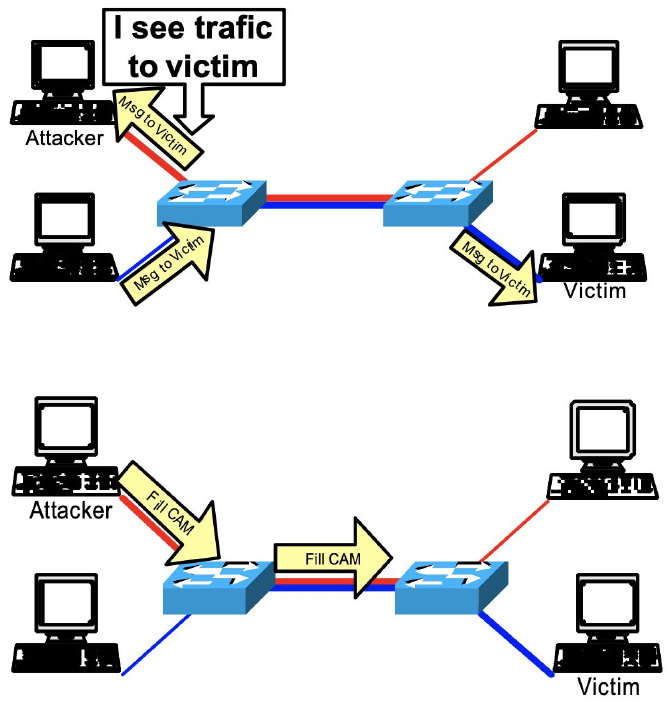
\includegraphics[scale=0.4]{../../immagini/MAC_flooding}
    \end{figure}
\\\\Per mitigare la vulnerabilità ci sono una serie di funzioni implementate nello switch, le \textbf{port security} features: questi permettono di specificare un indirizzo MAC per ogni porta o di imparare un certo numero di indirizzi MAC per porta.

\subsection{Basic VLAN Hopping attack}
L'hop vuol dire che si "salta" in una VLAN.
\\È un attacco base, la cui idea è che se un attacker riesce a connettersi ad una trunk port, può mandare un pacchetto in qualunque VLAN.
\\Il punto è riuscire a connettersi al trunk link: il protocollo DTP dei router CISCO è usato per negoziare il trunking su un link fra due device, ed il tipo di incapsulamento del trunking.
\\ Il problema è sempre che si può spoofare un pacchetto DTP per impersonare uno switch ed ottenere un trunk link.
\\Per mitigarlo, si può disabilitare DTP sulle porte che sappiamo non essere connesse a switch

\subsection{Double encapsulation}
È sempre un VLAN hopping attack, ma viene fatto incapsulando il pacchetto in due header 802.1Q.
\\L'attacco si basa sul fatto che gli switch \textit{VLAN aware} supportano la native VLAN, per comunicare con gli unaware switch.
\\Un pacchetto non taggato sul trunk link viene visto come un pacchetto dalla native VLAN: se viene ricevuto un pacchetto col tag della prossima native VLAN e deve essere forwardato ad un altro trunk link con valore della native VLAN, quell'header viene rimosso.
\\In situazioni particolari, la native VLAN può mandare pacchetti con questo double tag: il primo switch rimuove il primo tag, della native VLAN, il secondo rimuove quello più interno ed alla fine il pacchetto arriva alla vittima.
\\Un attacker deve essere attaccato ad una trunk port, oppure ad una access port che ha lo stesso ID della native VLAN, inoltre lo switch deve accettare pacchetti con i tag anche dalle access port.
\\Per evitare l'attacco, non bisognerebbe mai usare un VLAN ID come native VLAN.

\subsection{ARP attack}
Sempre lo stesso, non si può fare ad una vittima in un'altra VLAN ma si può comunque fare

\subsection{Spanning Tree Attack}
Ricordiamo che lo STP viene usato per mantenere la rete priva di loop in caso di topologia ridondante a layer 2.
\\I messaggi vengono inviati usando i Bridge Protocol Data Unit (BPDUs): l'attaccante che lo manda può forzare un root bridge a cambiare e quindi a creare un DoS nella rete.
\\L'attaccante può anche vedere delle trame che non dovrebbe poter vedere, inoltre esistono dei tool per poter replicare l'attacco, la richiesta per l'utilizzo è che l'attaccante sia dual-homed su due switch differenti.
\\Possibili contromisure:
\begin{itemize}
    \item disabilitare STP, ma non è una buona idea (l'introduzione di loop potrebbe divenire un'altra fonte di attacco);
    \item BDPU guard: disabilita le interfacce usando portfast per rilevare messaggi BDPU;
    \item Root guard disabilita le interfacce e diviene il bridge di root
\end{itemize}

\subsection{VLAN Trunking Protocol Attack}
VTP riduce l'amministrazione della rete con switch.
\\Quando viene configurata una nuova VLAN su un VTP server, la VLAN viene distribuita fra tutti gli switch del dominio.
\\VTP è un protocollo proprietario CISCO presente nella maggior parte dei prodotti: dopo aver negoziato la trunk port, l'attccante può mandare un messaggio VTP come server senza una VLAN configurata.
\\Per evitarlo, disabilitare VTP o usare almeno autenticazione con MD5.

\subsection{CDP attack}
Altro protocollo CISCO, i pacchetti sono in chiaro, c'era una vulnerabilità nei router CISCO che faceva andare oom e crashare.
\\Il CDP permette ai device di comunicare fra loro, quindi può essere usato per scoprire informazioni come idnrizzi IP, versione del software etc...
\\Come mitigazioni:
\begin{itemize}
    \item disabilitare CDP;
    \item essere molto selettivo nella scelta di usato in ambiente sensibile (da un punto di vista di sicurezza) 
\end{itemize}

\subsection{Private VLAN attack}
Possiamo definire una VLAN privata, abbiamo anche però i concetti di VLAN primarie e secondarie, ma i concetti sono sempre simili.
\\Abbiamo l'attacker in una VLAN privata, quindi la comunicazione non è possibile, per cui l'unico modo per comunicare è passare per il router e fare spoofing:\\
    \begin{figure}[h!]
        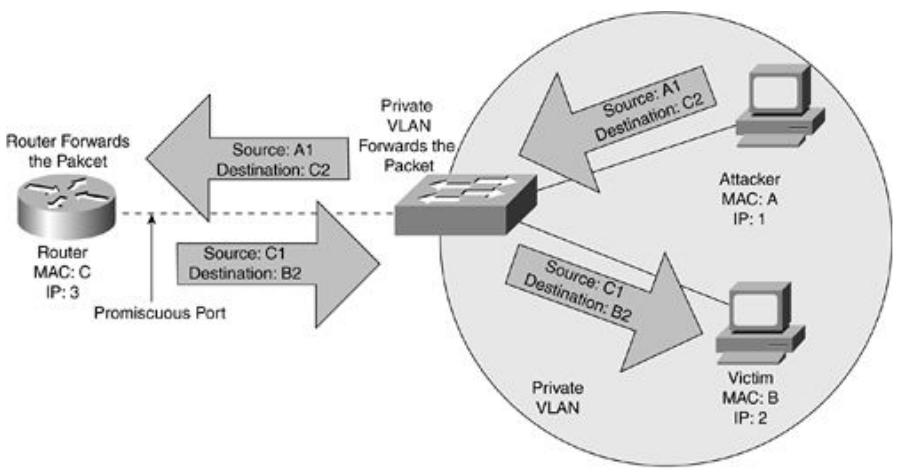
\includegraphics[scale=0.4]{../../immagini/pvlan_attack}
    \end{figure}
\\\\2 nel caso dell attacker è l'IP della vittima, la destinazione è il MAC del attacker. Stando attenti con le ACL è possibile evitare questo tipo di attacchi.

\section*{LAB 4}
La topologia è come quella del LAB3, ma su cumulus l'attacco del double incapsulation non funziona, perché la access port non accetta pacchetti taggati. È tipico che, magari si attiva una porta di uno switch e non si assegna una VLAN, e questa viene assegnata per default ad 1 che è proprio la VLAN native di default e quindi rende fattibile l'attacco.

\end{document}
